\documentclass[a4paper]{article}

% General style
\usepackage{newunicodechar}
\newunicodechar{→}{\fontspec{Gentium Plus}→}
\newunicodechar{–}{--}
\newunicodechar{“}{``}
\newunicodechar{”}{''}
\newunicodechar{‘}{`}
\newunicodechar{’}{'}

% Formulas
\usepackage{amsmath}
\usepackage{amssymb}

% Internal references
\usepackage{hyperref}
\usepackage[capitalize]{cleveref}

% Figures
\usepackage{subcaption}
\usepackage[font=small,labelfont=it]{caption}
\usepackage{graphicx}
\usepackage{tikz}
\usetikzlibrary{arrows}
\usetikzlibrary{arrows.meta}
\usetikzlibrary{decorations.pathreplacing}
\usetikzlibrary{bayesnet}
\usepackage[linguistics,edges]{forest}
\usepackage{rotating}

% Bibliography
\usepackage[backend=biber,
            bibstyle=numeric-comp, %biblatex-sp-unified,
            citestyle=numeric-comp,
            sorting=none,
            maxcitenames=2,url=false,
            maxbibnames=10]{biblatex}
\addbibresource{library.bib}
\def\bibfont{\fontfamily{\rmdefault}\fontseries{m}\fontshape{n}\fontsize{9}{11}\selectfont}

\renewbibmacro*{doi+eprint+url}{%
  \printfield{doi}%
  \newunit\newblock%
  \iftoggle{bbx:eprint}{%
    \usebibmacro{eprint}%
  }{}%
  \newunit\newblock%
  \iffieldundef{doi}{%
    \usebibmacro{url+urldate}}%
  {}%
}

\newcommand{\glot}[2]{#1 {\scriptsize{[\texttt{\href{https://glottolog.org/resource/languoid/id/#2}{#2}}]}}}

% Code inclusion with syntax highlighting
\usepackage{minted}
\setminted{fontsize=\tiny,baselinestretch=0.9}



\title{Supplementary material: Clocks with bursts: Phylogenetic inference of schismogenesis in language evolution}
\date{}
\author{
  Gereon A. Kaiping$^{1}$,
  Nico Neureiter$^{1}$\\[2ex]
  $^{1}$Geographic Information Science Center, Universität Zürich, CH
}

\begin{document}
\maketitle
\renewcommand{\thepage}{S\arabic{page}} 
\renewcommand{\thesection}{S\arabic{section}}  
\renewcommand{\thetable}{S\arabic{table}}  
\renewcommand{\thefigure}{S\arabic{figure}}
\renewcommand{\figurename}{Figure} 

\section{Tree heights}

\begin{figure}
    \centering
    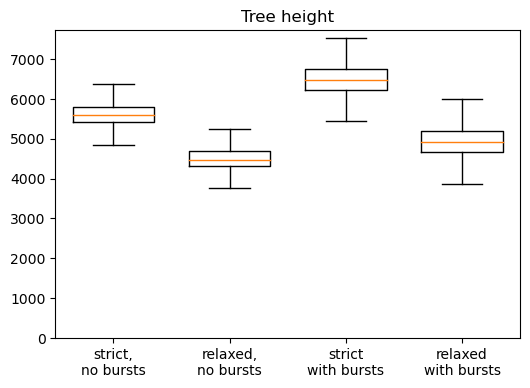
\includegraphics{supplement/analysis/austronesian_treeheight.png}
    \caption{The tree height/age of the Austronesian language family according to different clock models.}
    \label{fig:tree_height:austronesian}
\end{figure}

\begin{figure}
    \centering
    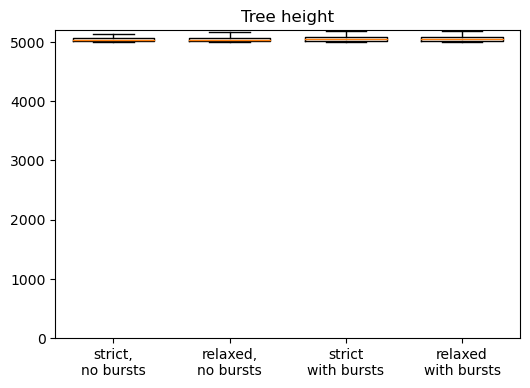
\includegraphics{supplement/analysis/bantu_treeheight.png}
    \caption{The tree height/age of the Bantu language family according to different clock models.}
    \label{fig:tree_height:bantu}
\end{figure}

\begin{figure}
    \centering
    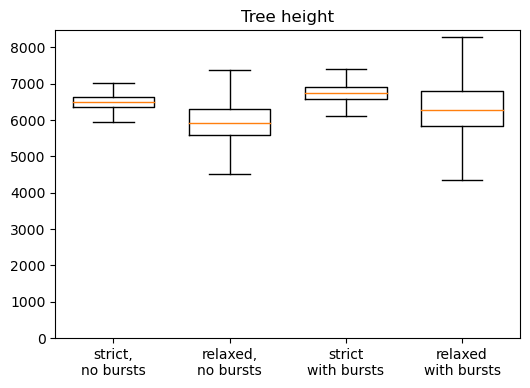
\includegraphics{supplement/analysis/indoeuropean_treeheight.png}
    \caption{The tree height/age of the Indo-European language family according to different clock models.}
    \label{fig:tree_height:indoeuropean}
\end{figure}

\begin{figure}
    \centering
    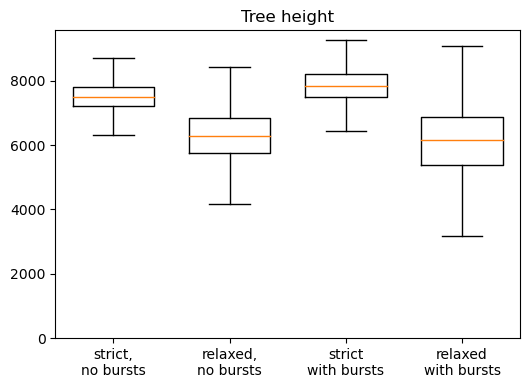
\includegraphics{supplement/analysis/sinotibetan_treeheight.png}
    \caption{The tree height/age of the Sino-Tibetan language family according to different clock models.}
    \label{fig:tree_height:sinotibetan}
\end{figure}


\section{Branch rate variation}

\begin{figure}
    \centering
    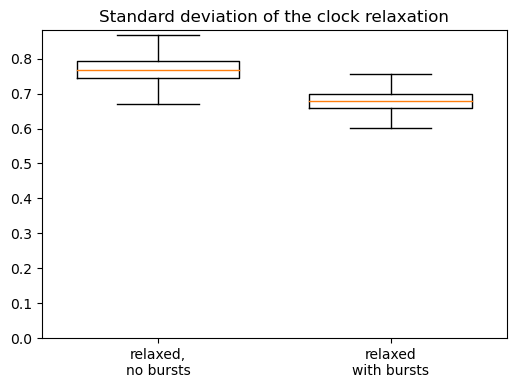
\includegraphics{supplement/analysis/austronesian_clockrates.png}
    \caption{The branch rate variation in the Austronesian language family with and without the burst clock.}
    \label{fig:rate_variation:austronesian}
\end{figure}

\begin{figure}
    \centering
    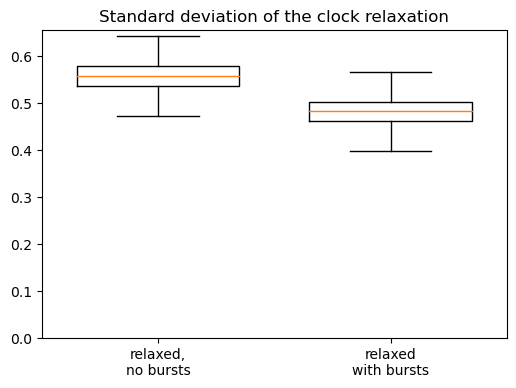
\includegraphics{supplement/analysis/bantu_clockrates.png}
    \caption{The branch rate variation in the Bantu language family with and without the burst clock.}
    \label{fig:rate_variation:bantu}
\end{figure}

\begin{figure}
    \centering
    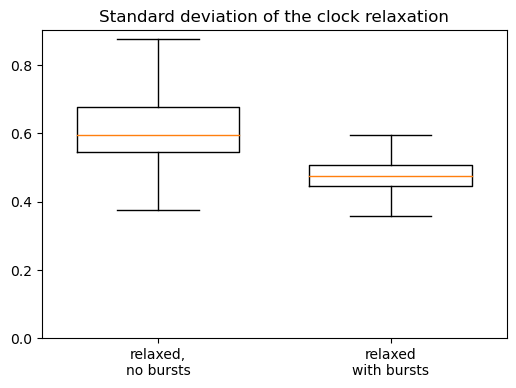
\includegraphics{supplement/analysis/indoeuropean_clockrates.png}
    \caption{The branch rate variation in the Indo-European language family with and without the burst clock.}
    \label{fig:rate_variation:indoeuropean}
\end{figure}

\begin{figure}
    \centering
    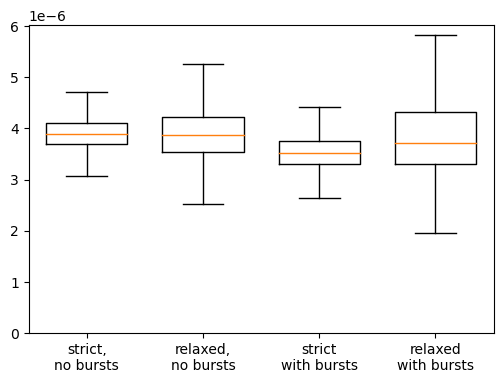
\includegraphics{supplement/analysis/sinotibetan_clockrates.png}
    \caption{The branch rate variation in the Sino-Tibetan language family with and without the burst clock.}
    \label{fig:rate_variation:sinotibetan}
\end{figure}

\end{document}